\documentclass[dvipdfmx,cjk]{beamer} 
\usepackage{graphicx}
\usepackage{tikz}
\usetheme{CambridgeUS} 

\AtBeginSection{\frame{\sectionpage}}
\AtBeginSubsection{\frame{\subsectionpage}}
\AtBeginSubsubsection{\frame{\subsubsectionpage}}

\begin{document}


\title[Halide]{ステンシル計算言語Halide}
\author[T. Muranushi]{村主崇行\\special thanks: 似鳥啓吾}            %% ここに書かれた情報は色々なところに使われるので
\institute[RIKEN/AICS]{計算科学研究機構}   %% なるべく設定した方が良い

\begin{frame}                  %% \begin{frame}..\end{frame} で 1 枚のスライド
\titlepage                     %% タイトルページ
\end{frame}

\begin{frame}                  %% 目次 (必要なければ省略)
\tableofcontents
\end{frame}

\section{はじめに} 

\begin{frame}\frametitle{ステンシル計算とは?}
配列変数を更新していくタイプのアルゴリズムで、配列の各要素を、それぞれ近傍の要素の値のみに基づき、同じルールで更新
するものをいう。

\pause

要するに

\pause

配列ベースの流体計算、MHD、等々
\end{frame}

\begin{frame}\frametitle{Halideとは?}
Halideはステンシル計算プログラムの生成とチューニングのためのライブラリ。
画像処理のために開発された。\cite{ragan2012decoupling,ragan2013halide}


\begin{center}
  \begin{tabular}{|c|c|c|}
    \hline
    &Paraiso & Halide\\
    \hline
    基本言語 & Haskell & C++ \\
    コード生成対象 & x86, CUDA &
    \multicolumn{1}{p{5cm}|}{x86/SSE, ARM, Native Client, OpenCL, CUDA,  ... }\\
    扱える次元 & n次元 & n次元 \\ 
    最適化の種類 & ループ融合、同期 & \multicolumn{1}{p{5cm}|}{並列度、局所性、計算節約 の間のトレードオフ} \\ 
    自動チューニング & あり & なし \\ 
    \hline
  \end{tabular}
\end{center}
\end{frame}

\section{Halideの文法} 
\begin{frame}[fragile]\frametitle{Halideの文法}

プログラミング言語Halideは、 C++のライブラリとして実装されている。

したがってHalideでプログラムするということはC++のプログラムを書くことになる。

基本的な型として、$n$次元配列を表す{\tt Func}と、配列添字変数を表す{\tt Var}
があり、これらを組み合わせてステンシル計算を記述する。

\pause

\begingroup
    \fontsize{8pt}{9pt}\selectfont
\begin{verbatim}
Func input = initial_condition.realize(NX,NY);
Var i,j;
Func cell2 = (input(i-1,j)+input(i,j)+input(i+1,j))/3;
Func output = (input(i,j-1)+input(i,j)+input(i,j+1))/3;
\end{verbatim}
\endgroup

\pause

以上のような構文を実現するため、C++の演算子オーバーロードを多用している。
例えば、複数引数関数のように見えるものは括弧演算子
{\tt operator()}をオーバーロードすることで
実現している。

\end{frame}


\begin{frame}[fragile]\frametitle{Halideのプログラムの例}

Halideではステンシル計算をとても直感的な形で記述することができる。

\pause

たとえば、以下のような拡散方程式の離散化解法は
\begin{eqnarray}
C_\mathrm{in} &=& \mathrm{initial~condition} \\
C_2 [i,j] &=& \frac{1}{3}\left(C_\mathrm{in}[i-1,j] + C_\mathrm{in}[i,j] + C_\mathrm{in}[i+1,j]\right) \\
C_\mathrm{out} [i,j] &=& \frac{1}{3}\left(C_\mathrm{2}[i,j-1] + C_\mathrm{2}[i,j] + C_\mathrm{2}[i,j+1]\right)
\end{eqnarray}

\pause

Halideではこのように記述できる。
\begin{center}
\begingroup
    \fontsize{9pt}{10pt}\selectfont
\begin{verbatim}
    Var i,j;
    Func input = initial_condition.realize(NX,NY);
    Func cell2 = (input(i-1,j)+input(i,j)+input(i+1,j))/3;
    Func output = (input(i,j-1)+input(i,j)+input(i,j+1))/3;
\end{verbatim}
\endgroup
\end{center}

\end{frame}


\begin{frame}[fragile]\frametitle{Halideのコード生成と実行}

Halideで配列変数としてもっとも頻繁に登場する
{\tt Func}型は、「その配列を計算するための手続き」を保持しているにすぎない。
これに対し{\tt Image}型は実際にメモリ上に確保された多次元配列である。

{\tt realize()}関数を呼び出して
{\tt Func}型を
{\tt Image}型に変換したとき、コード生成・最適化・実際の計算が行われる。
(プログラムに変更がなければ、いったん生成されたコードは使いまわされる)

\begingroup
    \fontsize{9pt}{10pt}\selectfont
\begin{verbatim}
    inPar.set(input);
    output=cell3.realize(NX,NY);
\end{verbatim}
\endgroup

\end{frame}

\begin{frame}[fragile]\frametitle{Halideにおけるステンシル計算の実装}
\begin{itemize}
\item {\tt Image}:実際にメモリ上に確保された配列
\item {\tt Func}:配列を操作するプログラムを構成するデータフローグラフの要素
\item {\tt ImageParam}:{\tt Image}へのポインタ、データフローグラフの入力点
\end{itemize}

\begin{center}
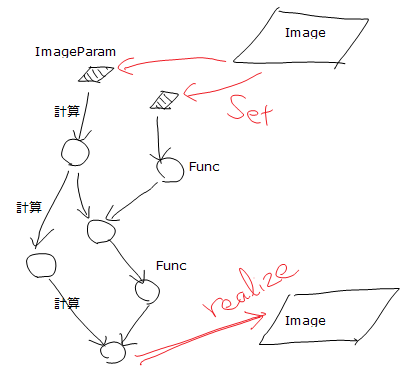
\includegraphics[height=4cm]{figure/DFG.png}
\end{center}
\end{frame}



\begin{frame}[fragile]\frametitle{Halideにおけるステンシル計算の実装例}

\begingroup
    \fontsize{9pt}{10pt}\selectfont
\begin{verbatim}
  Var x,y;             // 配列添字を表す変数
  Image input, output; // 計算結果を格納する配列変数
  ImageParam inPar;    // Halideプログラムの入力
  Func cell2 = a * inPar(x,y) + b * inPar(x+1,y); // Halideプログラム
  Func cell3 = c * cell2(x,y) + d * cell2(x,y+1); // Halideプログラム

  // 計算戦略を指定
  cell3.split(y, yo, yi, 16).parallel(yo).parallel(yo).vectorize(x,4);
  cell2.store_at(cell3,yo).compute_at(cell3,yi).vectorize(x,4);

  for (int t=0; t<=MAX_T; ++t) {
    inPar.set(input);             // プログラムに入力を設定
    output=cell3.realize(NX,NY);  // プログラムを実行
    std::swap(input, output);     // 出力を次のタイムステップの入力へ交換
  }


\end{verbatim}
\endgroup


\end{frame}


\begin{frame}[fragile]\frametitle{Halideのコード生成}

生成されたコードはその場で主プログラムにリンクされて実行される(Just in Time compile, JIT)
のほか、C++言語ソースやアセンブリ、LLVMバイトコードをファイルに生成させ、のちほど利用する(Ahead of Time compile, AOT)こともできる。

\begingroup
    \fontsize{9pt}{10pt}\selectfont
\begin{verbatim}
        compile_to_assembly
        compile_to_bitcode
        compile_to_c
        compile_to_file
        compile_to_function_pointers
        compile_to_header
        compile_to_lowered_stmt
        compile_to_native
        compile_to_object
        compile_to_src
\end{verbatim}
\endgroup

\end{frame}


\begin{frame}[fragile]\frametitle{コデザイン用コード生成言語としてのHalide/LLVM}

例えば、Halideから{\tt .bc}ファイルを生成した上で、Bulldozer向けアセンブリを生成させることで、
fma(融合加乗算)命令を含むアセンブリを生成できる。

\begingroup
    \fontsize{8pt}{9pt}\selectfont
\begin{verbatim}
$ clang -O1 -march=bdver1 -ffp-contract=fast blur.bc -S
$ less blur.s
...
	vfmaddss	%xmm3, (%r11,%rdi,4), %xmm1, %xmm3
	vfmaddss	%xmm3, (%r11,%r10,4), %xmm1, %xmm3
	vfmaddss	%xmm4, (%r11,%rax,4), %xmm1, %xmm4
	vfmaddss	%xmm4, (%r11,%r14,4), %xmm1, %xmm4
	vmulss	%xmm0, %xmm4, %xmm4
...
\end{verbatim}
\endgroup

これは将来のfmaをサポートするハードウェア向けのコード生成にも流用できると思われる。


\end{frame}


\section{Halideの最適化} 
\begin{frame}\frametitle{Halideの最適化空間}

Halideは、ステンシル計算の最適化問題を、
低並列度、演算重複、メモリ負荷、の間のトレードオフがある中で
計算とメモリの粒度を操作することで、計算の速度を最大化する
問題と捉えている。

計算とメモリの粒度とは何か?以下、拡散方程式を例に見ていく。

\begin{center}
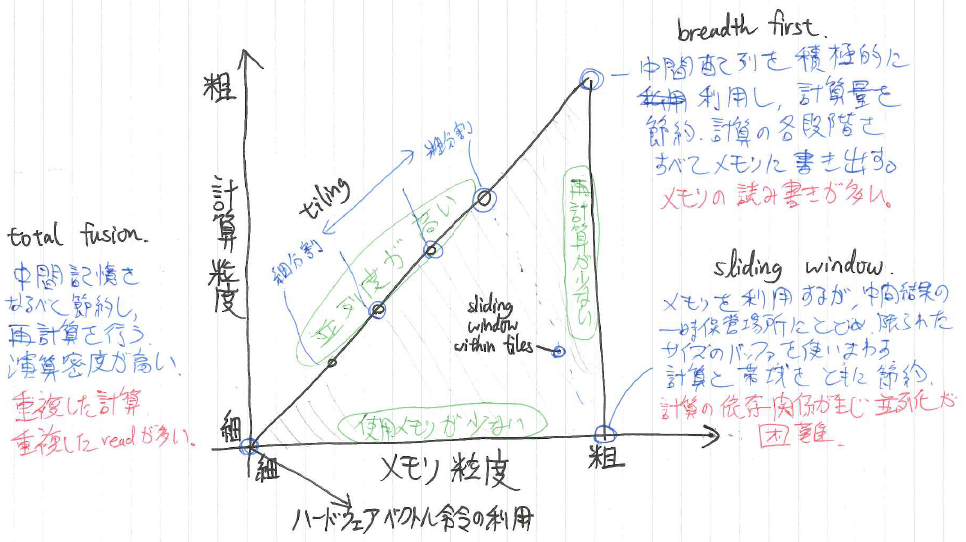
\includegraphics[width=8cm]{figure/doc/schedule-space.png}
\end{center}
\end{frame}


\begin{frame}\frametitle{Halideの最適化空間:粗メモリ、粗計算}

\begingroup \footnotesize
\begin{eqnarray*}
C_\mathrm{in} &=& \mathrm{initial~condition} \\
C_\mathrm{blurx} [i,j] &=& \frac{1}{3}\left(C_\mathrm{in}[i-1,j] + C_\mathrm{in}[i,j] + C_\mathrm{in}[i+1,j]\right) \\
C_\mathrm{out} [i,j] &=& \frac{1}{3}\left(C_\mathrm{2}[i,j-1] + C_\mathrm{2}[i,j] + C_\mathrm{2}[i,j+1]\right)
\end{eqnarray*}
\endgroup


\begin{center}
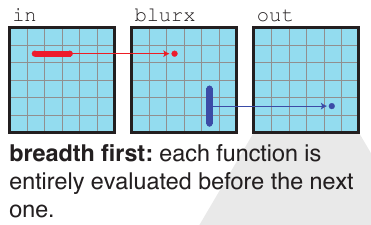
\includegraphics[width=4cm]{figure/doc/blur-breadth-first.png}
\end{center}


$C_\mathrm{blurx} [i,j]$ を全て計算し、メモリに置いてから、それを利用して
$C_\mathrm{out} [i,j]$を計算する。



\end{frame}


\begin{frame}\frametitle{Halideの最適化空間:細メモリ、細計算}

\begingroup \footnotesize
\begin{eqnarray*}
C_\mathrm{in} &=& \mathrm{initial~condition} \\
C_\mathrm{blurx} [i,j] &=& \frac{1}{3}\left(C_\mathrm{in}[i-1,j] + C_\mathrm{in}[i,j] + C_\mathrm{in}[i+1,j]\right) \\
C_\mathrm{out} [i,j] &=& \frac{1}{3}\left(C_\mathrm{2}[i,j-1] + C_\mathrm{2}[i,j] + C_\mathrm{2}[i,j+1]\right)
\end{eqnarray*}
\endgroup


\begin{center}
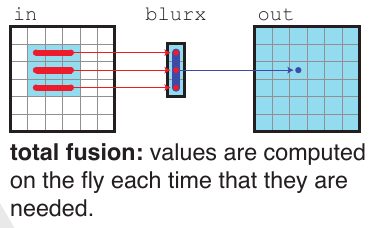
\includegraphics[width=4cm]{figure/doc/blur-fusion.png}
\end{center}

中間記憶を最低限しか使わず、$C_\mathrm{out} [i,j]$の各要素を計算するたびに、必要な$C_\mathrm{blurx} [i,j]$ の要素を全て再計算する。


\end{frame}

\begin{frame}\frametitle{Halideの最適化空間:粗メモリ、細計算}

% \begingroup \footnotesize
% \begin{eqnarray*}
% C_\mathrm{in} &=& \mathrm{initial~condition} \\
% C_\mathrm{blurx} [i,j] &=& \frac{1}{3}\left(C_\mathrm{in}[i-1,j] + C_\mathrm{in}[i,j] + C_\mathrm{in}[i+1,j]\right) \\
% C_\mathrm{out} [i,j] &=& \frac{1}{3}\left(C_\mathrm{2}[i,j-1] + C_\mathrm{2}[i,j] + C_\mathrm{2}[i,j+1]\right)
% \end{eqnarray*}
% \endgroup


\begin{center}
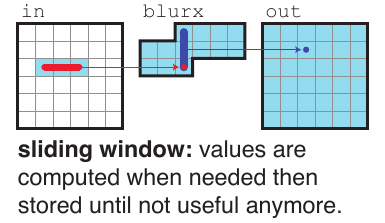
\includegraphics[width=4cm]{figure/doc/blur-sliding-window.png}
\end{center}

$C_\mathrm{out} [i,j]$の各要素を計算するたびに、新たな
$C_\mathrm{blurx} [i,j]$ の要素を計算するが、それを保持しておき再利用。
これ以上利用されなくなった時に破棄。中間結果をぴったり保持できるだけのバッファ
(この例だと3行分)を使いまわす。


\end{frame}


\begin{frame}\frametitle{粗メモリ粗計算と細メモリ細計算の中間}


\begin{center}
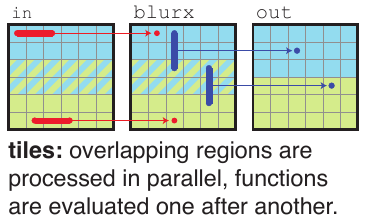
\includegraphics[width=4cm]{figure/doc/blur-tiles.png}
\end{center}

配列を1次元または2次元のタイルに分割し、タイル1個分を記憶できるだけのバッファを用意し、
その中ではすべての中間結果を保持する。タイルバッファを使いまわす。

タイルバッファのサイズがキャッシュに収まるときには高性能が期待できる。

\end{frame}

\begin{frame}\frametitle{すべての中間}


\begin{center}
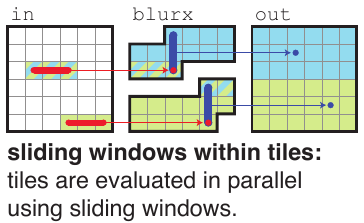
\includegraphics[width=4cm]{figure/doc/blur-sliding-within-tiles.png}
\end{center}

配列を1次元または2次元のタイルに分割し、タイル1個分を記憶できるだけのバッファを用意し、
その中では最低限のの中間結果を保持するバッファを使いまわす。
タイルごとの計算は並列に行う。



\end{frame}


\begin{frame}\frametitle{Halideの最適化空間}

\begin{center}
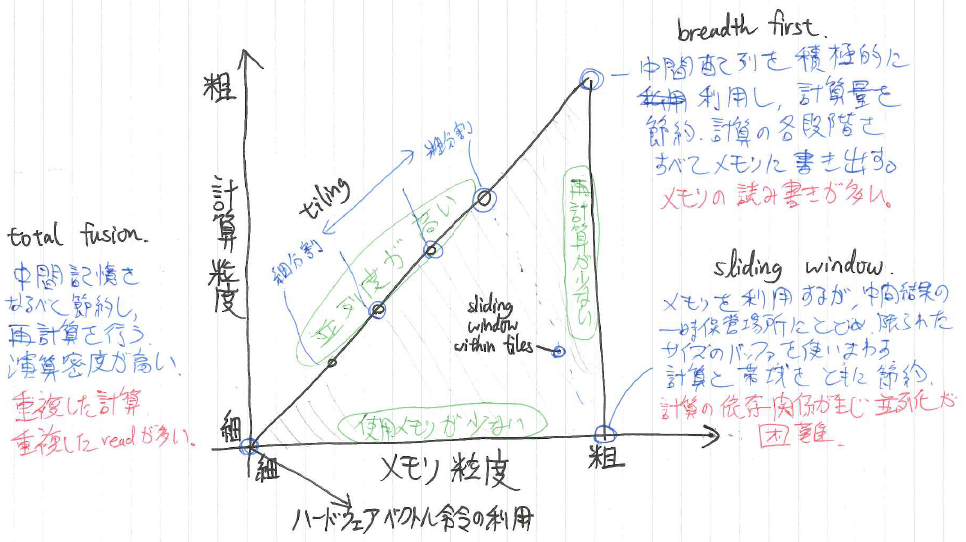
\includegraphics[width=12cm]{figure/doc/schedule-space.png}
\end{center}
\end{frame}



\begin{frame}\frametitle{Halideがサポートするプログラム変換の種類}

ステンシル計算の実装空間を探求するため、Halideはさまざまなプログラム変換をサポートする。

\begin{itemize}
  \item 分割:1..(M*N)までのループを1..Mと1..Nの二重ループに分割する
  \item 融合:1..Mと1..Nの2つのループを1つにまとめてしまう
  \item スレッド並列化:各添字を並列に計算
  \item アンロール:固定長のループを全部展開してループを消す
  \item ベクトル化:固定長のループをベクトル命令に置き換える
  \item タイル化:2次元のブロックを用意しそれを更新
  \item 入れ子ループの入れ替え
  \item 特殊化:条件変数が真の場合と偽の場合でループを分けループの中身を簡単化
\end{itemize}
\end{frame}



\begin{frame}[fragile]\frametitle{プログラム変換:ループ分割}

\begin{verbatim}
Func &split(Var old, Var outer, Var inner, Expr factor);
\end{verbatim}

配列変数添字{\tt old}のループアクセスを、
{\tt outer}と
{\tt inner}を添字とする二重ループに分割する。
内側のループ変数{\tt inner}が
{\tt [0 .. factor-1]}の範囲を動くように分割される。
\end{frame}

\begin{frame}[fragile]\frametitle{プログラム変換:ループ融合}


\begin{verbatim}
Func &fuse(Var inner, Var outer, Var fused);
\end{verbatim}

{\tt inner}と
{\tt outer}の二重ループを、
{\tt fused}を変数とする一重ループに融合する。
融合された変数の動く範囲の大きさは、もとの二つの変数の範囲の大きさの積になる。
\end{frame}

\begin{frame}[fragile]\frametitle{プログラム変換:並列化}

\begin{verbatim}
Func &parallel(Var var);
\end{verbatim}

変数{\tt var}を並列化。
{\tt var}の動く範囲の数だけのスレッドを立て(OpenMP)、
{\tt var}のそれぞれの値を並列に処理する。
\end{frame}

\begin{frame}[fragile]\frametitle{プログラム変換:アンロール}
\begin{verbatim}
Func &unroll(Var var);
Func &unroll(Var var, int factor);
\end{verbatim}

変数{\tt var}をアンロール。
{\tt var}のループを展開して消し、{\tt var}の値のすべての場合を逐次指定した
長いプログラムに変換する。
1引数版を使うには、{\tt var}の動く範囲が既知の定数である必要がある。
2引数版は、{\tt var}のループをサイズ{\tt factor}の内側ループと外側ループに
{\tt split}した上で内側をアンロールする。

\end{frame}

\begin{frame}[fragile]\frametitle{プログラム変換:ベクトル化}
\begin{verbatim}
Func &vectorize(Var var);
Func &vectorize(Var var, int factor);
\end{verbatim}

変数{\tt var}をベクトル化。
{\tt var}のループを無くして{\tt var}の値のすべての場合を一度の
ベクトル命令で処理する。
1引数版を使うには、{\tt var}の動く範囲が既知の定数である必要がある。
2引数版は、{\tt var}のループをサイズ{\tt factor}の内側ループと外側ループに
{\tt split}した上で内側をベクトル化する。
ベクトル長{\tt factor}がハードウェア側でサポートされてない場合の挙動は未調査。


\end{frame}

\begin{frame}[fragile]\frametitle{プログラム変換:タイル分割}

\begin{verbatim}
Func &tile(Var x, Var y,
           Var xo, Var yo,
           Var xi, Var yi,
           Expr xfactor, Expr yfactor);
\end{verbatim}

二つの添字{\tt x}と{\tt y}の二重ループアクセスを、
サイズ{\tt xfactor} $\times$
{\tt yfactor} のタイルに分割。
1つのタイル内をアクセスする添字{\tt xi}と{\tt yi}、および
タイルたちを参照する添字{\tt xo}と{\tt yo}の
四重ループに変換する。
\end{frame}



\section{ベンチマーク実験}
\begin{frame}\frametitle{ベンチマーク対象と環境}

以下のようなマシンで、拡散程式ソルバをスケジュールや問題サイズを変えて実行し、性能の変化を調べた。
似鳥さん、マシンを用意してくれてありがとう!

\begin{center}
  \begin{tabular}{|c|c|}
    \hline
    マシン名 & armagnac0\\
    CPU & AMD Opteron${}^\mathrm{(TM)}$ Processor 6376 \\
    freq & 1400MHz \\
    cores & 64 \\
    Memory & 256GB \\
    \hline
  \end{tabular}
\end{center}

\begin{itemize}
\item ノートPCだと一晩かかったLLVMのビルドが数分
\item {\tt llvm\$ make -j } fork爆弾事件
\end{itemize}
\end{frame}


\begin{frame}[fragile]\frametitle{ベンチマーク対象と環境}

シミュレーション対象アルゴリズム:

\begingroup \footnotesize
\begin{eqnarray*}
C_\mathrm{in} &=& \mathrm{initial~condition} \\
C_\mathrm{blurx} [i,j] &=& \frac{1}{3}\left(C_\mathrm{in}[i-1,j] + C_\mathrm{in}[i,j] + C_\mathrm{in}[i+1,j]\right) \\
C_\mathrm{out} [i,j] &=& \frac{1}{3}\left(C_\mathrm{2}[i,j-1] + C_\mathrm{2}[i,j] + C_\mathrm{2}[i,j+1]\right)
\end{eqnarray*}
\endgroup

問題サイズ$NX,NY$をそれぞれ$[16 .. 2^{15}]$まで変化させて(コード生成時間を含む)実行時間を測定する。

{\tt 1 core}:とくにコード変換なし

{\tt 64 core}:以下のコード変換を施す

\begingroup
    \fontsize{8pt}{9pt}\selectfont
\begin{verbatim}
  cell3.split(y, yo, yi, 16).parallel(yo).vectorize(x,4);
  cell2.store_at(cell3,yo).compute_at(cell3,yi).vectorize(x,4);
\end{verbatim}
\endgroup


\end{frame}

\begin{frame}[fragile]\frametitle{実行時間}
\begin{center}
\includegraphics[width=6cm,angle=270]{figure/result-wct.eps}
\end{center}
\end{frame}

\begin{frame}[fragile]\frametitle{実行効率}
\begin{center}
\includegraphics[width=6cm,angle=270]{figure/result-ef.eps}
\end{center}
\end{frame}

\section{Halideを用いた自動チューニング}

\begin{frame}\frametitle{マシンニンジャ計画}

\begin{itemize}
\item 実アプリ(具体的にはSeism3D)で
\item Ninjaが1週間くらいかけてチューニングしたのをうわまわる性能を
\item (京の100ノード×1週間くらいを消費する)自動チューニングにより達成すること
\end{itemize}


\begin{center}

\includegraphics[width=3cm]{figure/machine-ninja.jpg}
\end{center}
\end{frame}

\begin{frame}\frametitle{マシンニンジャ計画}
  Halideは、ステンシル計算を定義した上で様々なスケジュールを適用することで、生成プログラムの性能を様々にいじくれる、と主張していた。

  しかし、私がHalideのスケジュールの意味をよく理解していなかったのと、誤ったスケジュール(配列の範囲外アクセスなど)を設定してしまうとコード生成タイミングで実行時エラーになってしまい原因究明が困難であったことから、自由なスケジュール設定ができなかった。

  ところが、私がHalideのチュートリアルを全部追ったこと、およびHalideが、(ここ数日のバージョンアップで)無効なスケジュールを検出すると「有効なスケジュールの一覧」を出力するようになったことから、実行時エラーで落ちないスケジュールを自在に設定できるようになった。

  そこで、Halideのスケジュール空間を自動探索するプログラムを書いて走らせた(7月22日17:00〜)。
\end{frame}

\begin{frame}[fragile]\frametitle{Halideのスケジュールエラーメッセージの例}

無効なスケジュールを与えてしまった場合、Halideプログラムの実行時(コード生成時)に以下のようなエラーメッセージが出力される。

\begingroup \fontsize{8pt}{9pt}\selectfont
\begin{verbatim}
Function "cell3[2]" is computed and stored in the following invalid location:
cell3[2].compute_inline();
Legal locations for this function are:
cell3[2].compute_root();
cell3[2].store_root().compute_at(cell3[3], __outermost);
cell3[2].compute_at(cell3[3], __outermost);
cell3[2].compute_at(cell3[3], nid);
cell3[2].store_at(cell3[3], nid).compute_at(cell3[3], yi);
cell3[2].store_at(cell3[3], nid).compute_at(cell3[3], xi);
cell3[2].store_at(cell3[3], nid).compute_at(cell3[3], v129);
cell3[2].compute_at(cell3[3], yi);
cell3[2].store_at(cell3[3], yi).compute_at(cell3[3], xi);
cell3[2].store_at(cell3[3], yi).compute_at(cell3[3], v129);
cell3[2].compute_at(cell3[3], xi);
cell3[2].store_at(cell3[3], xi).compute_at(cell3[3], v129);
cell3[2].compute_at(cell3[3], v129);
cell3[2].compute_at(cell3[3], v128);
\end{verbatim}
\endgroup

\end{frame}


\begin{frame}\frametitle{Inter-timestep fusion}
  拡散方程式のプログラムは計算に比べてとてもメモリ負荷が大きい。
  理想的な場合でも1 load + 1 store あたり10演算なので、
  単精度として $0.8~B/F$。
  これに対し、armagnacの演算帯域比は、
  \begin{itemize}
  \item 演算: Opteron${}^\mathrm{(TM)}$ 6376は16コアで、1コアごとに128bit fma演算器が
    ついており、単精度は32bitで、fmaは2浮動小数演算(flop)ことを考慮すると128bit演算器でクロックあたり8flopこなせるから $\rm 8flop/core/clock \times 16 core/cpu \times 2.6GHz \times 4cpu = 1331.2GFlop/s$
  \item 帯域: 200GB/s (4 $\times$ 50GB/s)
  \end{itemize}
  
  とすると、$0.15~B/F$でどうしても足りない。
  
  アルゴリズム固有の限界0.8B/Fを超えて転送量を圧縮する方法として、
  複数の時間刻みを融合する方法が考えられる。$n$ステップを融合できれば、
  理想的な演算帯域比は
   $0.8/n~B/F$に近づけられるものと思われる。

\end{frame}


\begin{frame}\frametitle{チューニングパラメータの種別}
  Halideの生成するコードを制御するパラメータには以下のような種類がある。
  \begin{enumerate}
  \item  {\bf User option}: Inter-timestep fusionのような、配列変数の数を変えてしまうような変換
  \item  {\bf Loop option}ループ分割、融合、タイリングといったループの個数にまつわる選択肢(整数パラメータの個数を増やす可能性がある)
  \item  {\bf Timing option} 計算タイミング、ストアタイミングといった整数パラメータの個数を変えない選択肢
  \item  {\bf Int option}: ベクトル長、アンロール長といった整数パラメータの選択肢
    (Halideのscheduleの範囲に収まらないプログラム変換)
  \end{enumerate}
\end{frame}
  
\begin{frame}\frametitle{チューニングパラメータの種別}  
  Halideにおいてユーザが記述するC++プログラムは実際の数値計算プログラムの生成・実行ドライバに過ぎない。したがって、以上の選択肢はすべてC++の普通の値として表現すればよく、Halideを用いたプログラム実行速度最適化は、あたかもC++の普通の多引数関数の探索問題のように書くことができる。

  今回、User optionとしてはinter-timestep fusionの段数、Loop optionは固定とする。Timing optionはswitch文で選択。各種Int optionも探索する。
\end{frame}


\begin{frame}[fragile]\frametitle{オプションの列挙}

Halideプログラムはコードジェネレータなので、チューニングオプションはすべて通常の変数でよい。

\begingroup \fontsize{8pt}{9pt}\selectfont
\begin{verbatim}
int N_FUSION = 4;   // User option
int CELL2_CHOICE=4; // [0..8] Timing option
int CELL3_CHOICE=4; // [0..17] Timing option
int N_VECTOR=8;     // Int option
int N_UNROLL=4;     // Int option
int N_TILE_X=64;    // Int option
int N_TILE_Y=64;    // Int option
\end{verbatim}
\endgroup

\end{frame}


\begin{frame}[fragile]\frametitle{Inter-timestep fusionの実装}

{\tt N\_FUSION}段の時間ステップを融合するこうどなぷろぐらむも、ただのFor文として書ける。

\begingroup \fontsize{8pt}{9pt}\selectfont
\begin{verbatim}
  Halide::Func cell2[N_FUSION], cell3[N_FUSION];

  for(int i_f = 0; i_f < N_FUSION ; ++i_f) {
    if (i_f==0) {
      cell2[i_f](x,y)=a * inPar(x,y) + b * inPar(x+1,y) + b * inPar(x-1,y) ;
    } else {
      cell2[i_f](x,y)=a * cell3[i_f-1](x,y) + b *  cell3[i_f-1](x+1,y) + b * cell3[i_f-1](x-1,y);
    }
    cell3[i_f](x,y)= a * cell2[i_f](x,y) + b * cell2[i_f](x,y+1) + b * cell2[i_f](x,y-1) ;
  }
\end{verbatim}
\endgroup
\end{frame}



\begin{frame}[fragile]\frametitle{Timing optionの列挙}

先述のスケジュール無効メッセージから置換により生成したswitch文。

\begingroup \fontsize{8pt}{9pt}\selectfont
\begin{verbatim}
    switch(CELL2_CHOICE) {
    case 0 : cell2[i_f].compute_root(); break; 
    case 1 : cell2[i_f].store_root().compute_at(cell3[N_FUSION-1], Halide::Var::outermost()); break; 
    case 2 : cell2[i_f].compute_at(cell3[N_FUSION-1], Halide::Var::outermost()); break; 
    case 3 : cell2[i_f].compute_at(cell3[N_FUSION-1], nid); break; 
    case 4 : cell2[i_f].store_at(cell3[N_FUSION-1], nid).compute_at(cell3[N_FUSION-1], yi); break; 
    case 5 : cell2[i_f].store_at(cell3[N_FUSION-1], nid).compute_at(cell3[N_FUSION-1], xi); break; 
    case 6 : cell2[i_f].compute_at(cell3[N_FUSION-1], yi); break; 
    case 7 : cell2[i_f].store_at(cell3[N_FUSION-1], yi).compute_at(cell3[N_FUSION-1], xi); break; 
    default: cell2[i_f].compute_at(cell3[N_FUSION-1], xi); break; 
    }

    cell2[i_f].vectorize(x,N_VECTOR).unroll(x,N_UNROLL);
\end{verbatim}
\endgroup
\end{frame}

\begin{frame}[fragile]\frametitle{}
\begingroup \fontsize{8pt}{9pt}\selectfont
\begin{verbatim}
      switch(CELL3_CHOICE){
      case 0 : cell3[i_f].compute_root(); break;
      case 1 : cell3[i_f].store_root().compute_at(cell3[N_FUSION-1], Halide::Var::outermost()); break;
      case 2 : cell3[i_f].compute_at(cell3[N_FUSION-1], Halide::Var::outermost()); break;
      case 3 : cell3[i_f].compute_at(cell3[N_FUSION-1], nid); break;
      case 4 : cell3[i_f].store_at(cell3[N_FUSION-1], nid).compute_at(cell3[N_FUSION-1], yi); break;
      case 5 : cell3[i_f].store_at(cell3[N_FUSION-1], nid).compute_at(cell2[N_FUSION-1], Halide::Var::outermost()); break;
      case 6 : cell3[i_f].store_at(cell3[N_FUSION-1], nid).compute_at(cell2[N_FUSION-1], y); break;
      case 7 : cell3[i_f].store_at(cell3[N_FUSION-1], nid).compute_at(cell2[N_FUSION-1], x); break;
      case 8 : cell3[i_f].compute_at(cell3[N_FUSION-1], yi); break;
      case 9 : cell3[i_f].store_at(cell3[N_FUSION-1], yi).compute_at(cell2[N_FUSION-1], Halide::Var::outermost()); break;
      case 10 : cell3[i_f].store_at(cell3[N_FUSION-1], yi).compute_at(cell2[N_FUSION-1], y); break;
      case 11 : cell3[i_f].store_at(cell3[N_FUSION-1], yi).compute_at(cell2[N_FUSION-1], x); break;
      case 12 : cell3[i_f].compute_at(cell2[N_FUSION-1], Halide::Var::outermost()); break;
      case 13 : cell3[i_f].store_at(cell2[N_FUSION-1], Halide::Var::outermost()).compute_at(cell2[N_FUSION-1], y); break;
      case 14 : cell3[i_f].store_at(cell2[N_FUSION-1], Halide::Var::outermost()).compute_at(cell2[N_FUSION-1], x); break;
      case 15 : cell3[i_f].compute_at(cell2[N_FUSION-1], y); break;
      case 16 : cell3[i_f].store_at(cell2[N_FUSION-1], y).compute_at(cell2[N_FUSION-1], x); break;
      default : cell3[i_f].compute_at(cell2[N_FUSION-1], x); break;
      }

      cell3[i_f].vectorize(x,N_VECTOR).unroll(x,N_UNROLL);
\end{verbatim} 
\endgroup
\end{frame}


\begin{frame}[fragile]\frametitle{Halideのスケジュール空間探索まとめ}

Loop optionの設定

\begingroup \fontsize{8pt}{9pt}\selectfont
\begin{verbatim}
cell3[i_f].tile(x,y, xo,yo, xi, yi, N_TILE_X, N_TILE_Y) // タイル分割
          .fuse(xo,yo,nid) // タイルを識別する外側添字はx,yまとめてナンバリング
          .parallel(nid)   // そのタイルごとに並列化
          .vectorize(xi,N_VECTOR) // 再内側添字xiはまずN_VECTOR個づつベクトル化
          .unroll(xi,N_UNROLL);   // さらにN_UNROLL個づつアンロール
\end{verbatim}
\endgroup

User optionとInt option

\begingroup \fontsize{8pt}{9pt}\selectfont
\begin{verbatim}
int N_FUSION = 4;   // [1..32]  User option   : Inter-timestep fusionの段数
int CELL2_CHOICE=4; // [0..8]   Timing option : cell2(y差分)のタイミング
int CELL3_CHOICE=4; // [0..17]  Timing option : cell3(x差分)のタイミング
int N_VECTOR=8;     // [1..8]   Int option    : マシンベクトル長
int N_UNROLL=4;     // [1..32]  Int option    : アンロール段数
int N_TILE_X=64;    // [1..512] Int option    : タイルバッファのサイズ(x)
int N_TILE_Y=64;    // [1..512] Int option    : タイルバッファのサイズ(y)
\end{verbatim}
\endgroup

\begingroup \fontsize{8pt}{9pt}\selectfont
\begin{verbatim}
[全オプションを]
↓
\end{verbatim}
\endgroup
\end{frame}


\begin{frame}[fragile]\frametitle{Bench result}
\begin{center}
\includegraphics[height=9.7cm,angle=270]{figure/bench_fusion.eps}
\end{center}
\end{frame}
\begin{frame}[fragile]\frametitle{Bench result}
\begin{center}
\includegraphics[height=9.7cm,angle=270]{figure/bench_space_size.eps}
\end{center}
\end{frame}
\begin{frame}[fragile]\frametitle{Bench result}
\begin{center}
\includegraphics[height=9.7cm,angle=270]{figure/bench_timestep.eps}
\end{center}
\end{frame}
\begin{frame}[fragile]\frametitle{Bench result}
\begin{center}
\includegraphics[height=9.7cm,angle=270]{figure/bench_ulen.eps}
\end{center}
\end{frame}
\begin{frame}[fragile]\frametitle{Bench result}
\begin{center}
\includegraphics[height=9.7cm,angle=270]{figure/bench_vlen.eps}
\end{center}
\end{frame}



\begin{frame}\frametitle{Halideの自動性能探索まとめ}
\begin{itemize}
\item Halideが生成するコードはなぜか整数命令が多すぎる
\item イントリンシックを並べるのがよいです。
\item 明日前田先生に会いにいきます@東京
\end{itemize}

\end{frame}




\begin{frame}[allowframebreaks]{参考文献}{}
  \bibliographystyle{apalike}
  \bibliography{bunken}
\end{frame}



% \begin{bibliography}
% 
% \bibitem[de~Saussure, 1995]{Saussure1995}
% de~Saussure, F. (1995).
% \newblock {\em Cours de Linguistique Grale}.
% \newblock Payot.
% 
% \bibitem[Labov, 1972]{Labov1972}
% Labov, W. (1972).
% \newblock {\em Sociolinguistic Patterns}.
% \newblock University of Pennsylvania Press, Philadelphia.
% 
% \end{bibliography}








\section*{リサイクルボックス}




\subsection{}
\begin{frame}\frametitle{}
\begin{eqnarray}
\end{eqnarray}
\end{frame}


\begin{frame}[fragile]\frametitle{}
\begingroup \fontsize{8pt}{9pt}\selectfont
\begin{verbatim}
subroutine kernel__velderiv()
\end{verbatim}
\endgroup
\end{frame}




\end{document}

